\documentclass[../views.tex]{subfiles}

\begin{document}

Een process view omvat de draaiende processen van een programma. Het omschrijft hoe processen met elkaar samenwerken, zowel intern als extern \parencite{architectural_blueprints}. Een versimpeld proces omvat meer processen, maar worden weergegeven als één proces. De process views zijn te vinden in \autoref{fig:process_view_server}, \ref{fig:process_view_collector} en \ref{fig:process_view_frontend}.

% server
\begin{figure}[ht]
  \centering
  \fbox{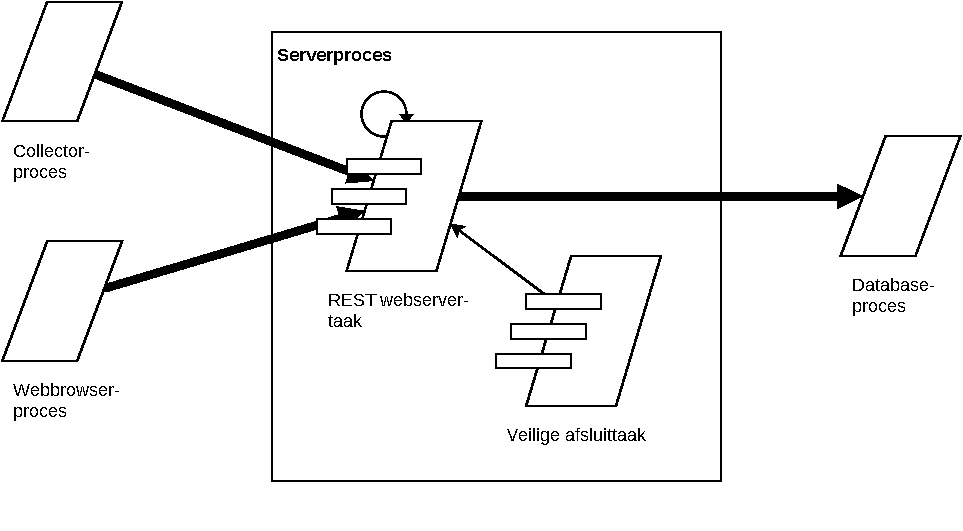
\includegraphics[width=0.95\textwidth]{../assets/images/drawio/process view server.pdf}}
  \caption{Process view server.}
  \label{fig:process_view_server}
\end{figure}

% collector
\begin{figure}[ht]
  \centering
  \fbox{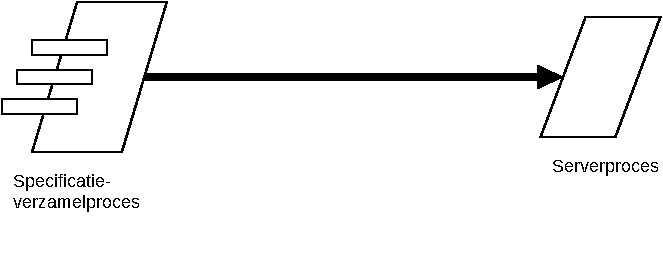
\includegraphics[width=0.5\textwidth]{../assets/images/drawio/process view collector.pdf}}
  \caption{Process view collector.}
  \label{fig:process_view_collector}
\end{figure}

% frontend
\begin{figure}[ht]
  \centering
  \fbox{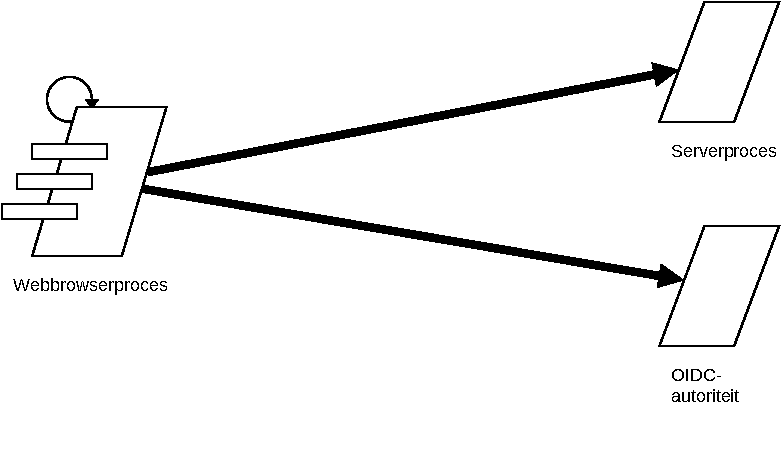
\includegraphics[width=0.95\textwidth]{../assets/images/drawio/process view frontend.pdf}}
  \caption{Process view frontend.}
  \label{fig:process_view_frontend}
\end{figure}

% Legenda
\begin{figure}[ht]
  \centering
  \fbox{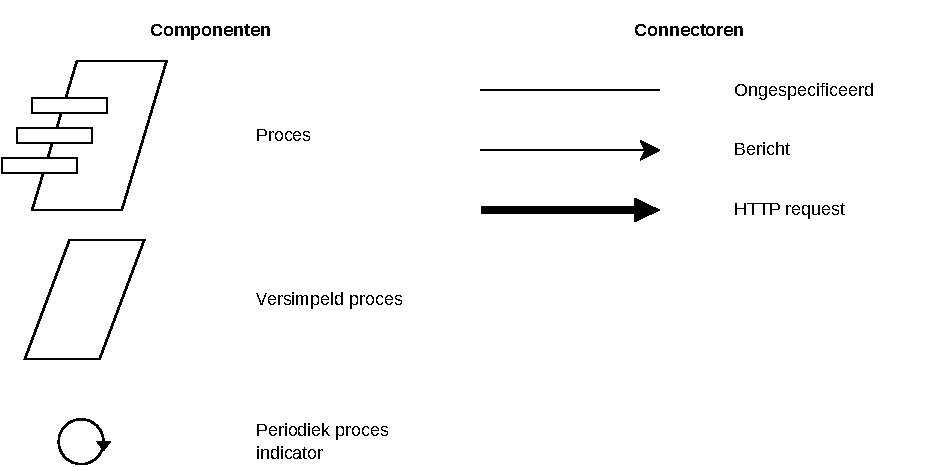
\includegraphics[width=0.95\textwidth]{../assets/images/drawio/process view legend.pdf}}
  \caption{Legenda voor de process views.}
\end{figure}

\end{document}
